% AUTO-GENERATED by scripts/make_preview.py -- do not edit; edit figures/*.tex and re-run the script.
% Preview of all figures in one compile. The per-figure PDFs still come from compiling each figures/figNN_*.tex.
\documentclass[10pt]{article}
\usepackage[letterpaper,margin=0.5in]{geometry}
\usepackage[T1]{fontenc}
\usepackage{newtxtext,newtxmath}
\usepackage{tikz}
\usepackage{pgfplots}
\pgfplotsset{compat=1.17}
\usetikzlibrary{arrows.meta,calc,positioning}
\definecolor{acc}{RGB}{31,78,121}
\colorlet{accfill}{acc!10}
\colorlet{gfill}{black!7}
\pagestyle{empty}
\setlength{\parindent}{0pt}
\begin{document}
\clearpage
{\noindent\textbf{fig01\_blind\_spot.tex}\hfill\textit{one column (3.5 in)}\par\medskip
{\tikzset{
  every node/.style={font=\footnotesize},
  cell/.style={draw=black,line width=0.5pt,fill=white,align=center,inner sep=2pt,
               minimum width=94pt,minimum height=16pt},
  tall/.style={minimum height=24pt},
  gray cell/.style={fill=gfill},
  acc cell/.style={draw=acc,fill=accfill,line width=0.7pt},
  rowlab/.style={anchor=east,align=right,inner sep=0pt},
}
\begin{tikzpicture}[x=1pt,y=1pt]
  % column headers
  \node at (97,2)  {\textbf{(a) Genuine feed}};
  \node at (197,2) {\textbf{(b) Decoy swap}};

  % ---- inputs to the two channels
  \node[rowlab] at (44,-24) {Banner};
  \node[rowlab] at (44,-50) {$T_{\mathrm{cve}}$};
  \node[rowlab] at (44,-74) {$s$};

  \node[cell,tall] at (97,-24)  {1080p, H.264\\ports 80, 554, 8000};
  \node[cell]      at (97,-50)  {$100$};
  \node[cell]      at (97,-74)  {$0.98$};

  \node[cell,tall] at (197,-24) {480p, MJPEG\\port 8080 only};
  \node[cell]      at (197,-50) {$100$};
  \node[cell,acc cell] at (197,-74) {$0.18$};

  % separator between inputs and decisions
  \draw[black!50,line width=0.4pt,dash pattern=on 2pt off 2pt] (0,-90) -- (248,-90);

  % ---- decisions
  \node[rowlab] at (44,-110) {CVE-only};
  \node[rowlab] at (44,-140) {IG-DCTF};

  \node[cell,tall,gray cell] at (97,-110)  {$T_{\mathrm{cve}}=100$\\high trust};
  \node[cell,tall]           at (97,-140)  {$T_{\mathrm{cve}}G(s)=100$\\high trust};

  \node[cell,tall,gray cell] at (197,-110) {$T_{\mathrm{cve}}=100$\\high trust};
  \node[cell,tall,acc cell]  at (197,-140) {$T_{\mathrm{cve}}G(s)=30$\\low trust};
\end{tikzpicture}
}}

\clearpage
{\noindent\textbf{fig02\_architecture.tex}\hfill\textit{full width (7.16 in)}\par\medskip
{\tikzset{
  >={Stealth[length=3pt,width=2.6pt]},
  every node/.style={font=\footnotesize},
  blk/.style={draw=black,line width=0.5pt,fill=white,align=center,inner sep=2pt,minimum height=24pt},
  inp/.style={blk,fill=gfill,minimum width=88pt},
  chan/.style={blk,minimum width=56pt},
  outp/.style={blk,minimum width=104pt},
  accblk/.style={draw=acc,fill=accfill,line width=0.7pt},
  grpbox/.style={draw=black!60,line width=0.5pt,dash pattern=on 2.5pt off 2pt},
  accgrpbox/.style={draw=acc,line width=0.5pt,dash pattern=on 2.5pt off 2pt},
  flow/.style={->,line width=0.5pt},
  ftitle/.style={anchor=south west,inner sep=1pt,font=\footnotesize\bfseries},
}
\begin{tikzpicture}[x=1pt,y=1pt]

  % ---------------- inputs
  \node[inp,minimum height=28pt] (inNVD)  at (48,-46)  {NVD, CISA KEV,\\EPSS, WHOIS};
  \node[inp,minimum height=28pt] (inSho)  at (48,-104) {Shodan / Censys\\banners (passive)};
  \node[inp,minimum height=28pt] (inVid)  at (48,-184) {Authorized footage\\(YOLOv8, ByteTrack)};

  % ---------------- Channel A
  \draw[grpbox] (108,-6) rectangle (308,-86);
  \node[ftitle] at (110,-6) {Channel A: cyber posture};
  \node[chan] (A1) at (142,-30) {Authentication\\(banner)};
  \node[chan] (A2) at (206,-30) {CVE class\\(CWE map)};
  \node[chan] (A3) at (142,-62) {Owner,\\patch age};
  \node[chan] (A4) at (206,-62) {Corroboration\\(neighbours)};
  \node[blk,minimum width=58pt] (Tc) at (272,-46) {Cyber trust\\$T_{\mathrm{cve}}$};
  \draw[flow] (A2.east) -| (Tc.north);
  \draw[flow] (A4.east) -| (Tc.south);

  % ---------------- Channel B
  \draw[accgrpbox] (108,-122) rectangle (308,-202);
  \node[ftitle,text=acc] at (110,-122) {Channel B: signal authenticity};
  \node[chan,accblk,minimum width=104pt,minimum height=28pt] (B1) at (168,-148) {Tier 1: banner drift\\(all devices, passive)};
  \node[chan,accblk,minimum width=104pt,minimum height=28pt] (B2) at (168,-184) {Tier 2: frame liveness\\(authorized feeds only)};
  \node[blk,accblk,minimum width=58pt,minimum height=28pt] (Sg) at (272,-166) {Integrity\\$s$};
  \draw[flow] (B1.east) -| (Sg.north);
  \draw[flow] (B2.east) -| (Sg.south);
  \draw[flow] (B1.south) -- (B2.north);

  % ---------------- gate
  \node[blk,accblk,minimum width=66pt,minimum height=44pt] (G) at (356,-106) {Gate\\$T_{\mathrm{cve}}\,G(s)$};
  \draw[flow] (Tc.east) -| (G.north);
  \draw[flow] (Sg.east) -| (G.south);

  % ---------------- outputs
  \node[outp] (O1) at (462,-40)  {Tiered dispatch\\emergency, triage, silent};
  \node[outp] (O2) at (462,-106) {Merkle audit ledger\\(+ gate-trip entry)};
  \node[outp] (O3) at (462,-172) {Dashboard (WebSocket)\\gate-trip events};
  \draw[flow] (G.east) -- (O2.west);
  \draw[flow] (G.east) -- ++(10,0) |- (O1.west);
  \draw[flow] (G.east) -- ++(10,0) |- (O3.west);

  % ---------------- inputs -> channels
  \draw[flow] (inNVD.east) -- (108,-46);
  \draw[flow] (inSho.east) -- ++(7,0) |- (108,-72);
  \draw[flow] (inSho.east) -- ++(7,0) |- (108,-136);
  \draw[flow] (inVid.east) -- (B2.west);
\end{tikzpicture}
}}

\clearpage
{\noindent\textbf{fig03\_threat\_model.tex}\hfill\textit{one column (3.5 in)}\par\medskip
{\tikzset{
  >={Stealth[length=3pt,width=2.6pt]},
  every node/.style={font=\footnotesize},
  col1/.style={draw=black,line width=0.5pt,fill=gfill,align=left,inner sep=2.5pt,
               text width=66pt,minimum height=34pt},
  col2/.style={draw=black,line width=0.5pt,fill=white,align=left,inner sep=2.5pt,
               text width=56pt,minimum height=34pt},
  col3/.style={draw=acc,line width=0.7pt,fill=accfill,align=left,inner sep=2.5pt,
               text width=74pt,minimum height=34pt},
  head/.style={align=center,font=\footnotesize\bfseries},
  flow/.style={->,line width=0.5pt},
}
\begin{tikzpicture}[x=1pt,y=1pt]
  % headers (column centres: 36, 127, 214)
  \node[head] at (36,0)  {Adversary};
  \node[head] at (126,0) {Entry point};
  \node[head] at (211,0) {Countermeasure};

  % rows
  \node[col1] (r1a) at (36,-28)  {$\mathcal{A}_1$ Decoy swap or MITM relay};
  \node[col2] (r1b) at (126,-28) {Device endpoint, RTSP relay};
  \node[col3] (r1c) at (211,-28) {Tier 1 drift; Tier 2 spec check};

  \node[col1] (r2a) at (36,-68)  {$\mathcal{A}_2$ Stream freeze or loop};
  \node[col2] (r2b) at (126,-68) {RTSP video stream};
  \node[col3] (r2c) at (211,-68) {Tier 2 pHash freeze, blur drift};

  \node[col1] (r3a) at (36,-108)  {$\mathcal{A}_3$ Collusive corroboration};
  \node[col2] (r3b) at (126,-108) {Adjacency graph, event API};
  \node[col3] (r3c) at (211,-108) {Velocity tracker, graph analysis};

  \node[col1] (r4a) at (36,-148)  {$\mathcal{A}_4$ Metadata spoofing};
  \node[col2] (r4b) at (126,-148) {Detection-event payload};
  \node[col3] (r4c) at (211,-148) {DB-sourced attributes, API key, replay checks};

  \foreach \i in {1,2,3,4}{
    \draw[flow] (r\i a.east) -- (r\i b.west);
    \draw[flow] (r\i b.east) -- (r\i c.west);
  }
\end{tikzpicture}
}}

\clearpage
{\noindent\textbf{fig04\_tier1\_drift.tex}\hfill\textit{one column (3.5 in)}\par\medskip
{\tikzset{
  >={Stealth[length=3pt,width=2.6pt]},
  every node/.style={font=\footnotesize,inner sep=0pt},
  c0/.style={anchor=west},
  c1/.style={anchor=west},
  c2/.style={anchor=west},
  c3/.style={anchor=east},
  c4/.style={anchor=east},
  chg/.style={text=acc},          
  rule/.style={line width=0.5pt,black},
}
\begin{tikzpicture}[x=1pt,y=1pt]
  % column anchors: field 0, baseline 50, current 120, delta (right edge) 198, weight (right edge) 228
  \draw[rule] (-2,8) -- (230,8);
  \node[c0] at (0,0)   {Field};
  \node[c1] at (50,0)  {$\mathcal{B}_d(t{-}1)$};
  \node[c2] at (120,0) {$\mathcal{B}_d(t)$};
  \node[c3] at (198,0) {$\delta_i$};
  \node[c4] at (228,0) {$w_i$};
  \draw[rule] (-2,-7) -- (230,-7);

  % rows (pitch 13 pt)
  \node[c0] at (0,-15)  {Product};
  \node[c1] at (50,-15) {ds-2cd2042wd-i};
  \node[c2] at (120,-15){ds-2cd2042wd-i};
  \node[c3] at (198,-15){$0$};
  \node[c4] at (228,-15){$0.10$};

  \node[c0] at (0,-28)  {HTTP server};
  \node[c1] at (50,-28) {hikvision-webs};
  \node[c2,chg] at (120,-28){micro\_httpd};
  \node[c3] at (198,-28){$1$};
  \node[c4] at (228,-28){$0.20$};

  \node[c0] at (0,-41)  {Firmware};
  \node[c1] at (50,-41) {v5.5.80};
  \node[c2,chg] at (120,-41){v1.0};
  \node[c3] at (198,-41){$1$};
  \node[c4] at (228,-41){$0.25$};

  \node[c0] at (0,-54)  {Open ports};
  \node[c1] at (50,-54) {$\{80,554,8000\}$};
  \node[c2,chg] at (120,-54){$\{8080\}$};
  \node[c3] at (198,-54){$1.00$};
  \node[c4] at (228,-54){$0.20$};

  \node[c0] at (0,-67)  {Resolution};
  \node[c1] at (50,-67) {1080p};
  \node[c2,chg] at (120,-67){480p};
  \node[c3] at (198,-67){$1$};
  \node[c4] at (228,-67){$0.20$};

  \node[c0] at (0,-80)  {Codec};
  \node[c1] at (50,-80) {H.264};
  \node[c2] at (120,-80){H.264};
  \node[c3] at (198,-80){$0$};
  \node[c4] at (228,-80){$0.05$};

  \draw[rule] (-2,-88) -- (230,-88);

  % result
  \node[anchor=west] at (0,-100) {$\mathrm{Drift}(d,t)=\sum_i w_i\,\delta_i = 0.85$};
  \node[anchor=west,text=acc] at (0,-114) {$s = 1-0.85 = 0.15 < \theta_{\mathrm{low}}$: gate tripped, $G=0.30$};
\end{tikzpicture}
}}

\clearpage
{\noindent\textbf{fig05\_tier2\_liveness.tex}\hfill\textit{full width (7.16 in)}\par\medskip
{\tikzset{
  >={Stealth[length=3pt,width=2.6pt]},
  every node/.style={font=\footnotesize},
  st/.style={draw=black,line width=0.5pt,fill=white,align=center,inner sep=2pt,minimum height=28pt},
  s1/.style={st,minimum width=76pt},
  s2/.style={st,minimum width=84pt},
  s3/.style={st,minimum width=84pt,fill=gfill},
  frm/.style={st,minimum width=34pt,fill=gfill},
  agg/.style={draw=acc,line width=0.7pt,fill=accfill,align=center,inner sep=2pt,minimum height=28pt,minimum width=74pt},
  flow/.style={->,line width=0.5pt},
  wlab/.style={anchor=south,inner sep=1pt},
}
\begin{tikzpicture}[x=1pt,y=1pt]
  % boundary of the authorised-footage-only region
  \draw[dashed,line width=0.5pt,black!60] (2,-124) rectangle (510,22);
  \node[anchor=south west,inner sep=1pt,font=\footnotesize\bfseries] at (4,22) {Tier 2: authorized footage only};

  % input frame
  \node[frm] (F) at (24,-50) {Frame\\$f_t$};

  % branch 1: freeze
  \node[s1] (a1) at (94,0)    {pHash, Hamming\\distance to $f_{t-1}$};
  \node[s2] (a2) at (192,0)   {Run length $c$ of\\frames with $d\le 1$};
  \node[s3] (a3) at (288,0)   {$\mathrm{Freeze}=[\,c\ge 25\,]$};

  % branch 2: quality drift
  \node[s1] (b1) at (94,-50)  {Variance of\\Laplacian $v_t$};
  \node[s2] (b2) at (192,-50) {EWMA baseline $\mu_t$\\($\alpha=0.05$)};
  \node[s3] (b3) at (288,-50) {$q=\mathrm{clip}(1-v_t/\mu_t)$};

  % branch 3: spec mismatch
  \node[s1] (c1) at (94,-100)  {Frame size\\$W\times H$};
  \node[s2] (c2) at (192,-100) {Compare with Tier 1\\declared resolution};
  \node[s3] (c3) at (288,-100) {$m\in\{0,1\}$};

  % aggregation
  \node[agg] (mx) at (413,-50) {$L=1-\max(\cdot)$\\of weighted terms};

  % flows: frame to the three branches
  \draw[flow] (F.east) -- ++(9,0) |- (a1.west);
  \draw[flow] (F.east) -- (b1.west);
  \draw[flow] (F.east) -- ++(9,0) |- (c1.west);
  \foreach \r in {a,b,c}{
    \draw[flow] (\r1.east) -- (\r2.west);
    \draw[flow] (\r2.east) -- (\r3.west);
  }
  % flows: weighted bus into the aggregator
  \draw[flow] (a3.east) -- ++(24,0) |- (mx.west);
  \draw[flow] (b3.east) -- (mx.west);
  \draw[flow] (c3.east) -- ++(24,0) |- (mx.west);
  \node[wlab] at (342,0)    {$\times 1.0$};
  \node[wlab] at (342,-50)  {$\times 0.6$};
  \node[wlab] at (342,-100) {$\times 0.5$};

  % output
  \draw[flow] (mx.east) -- ++(26,0) node[right,inner sep=2pt] {$L(t)$};
\end{tikzpicture}
}}

\clearpage
{\noindent\textbf{fig06\_gate\_function.tex}\hfill\textit{one column (3.5 in)}\par\medskip
{
\footnotesize
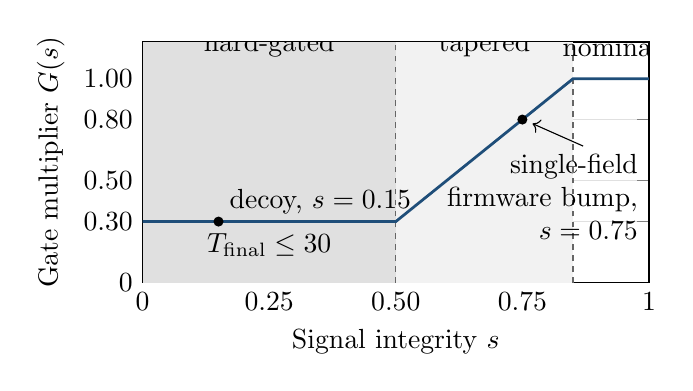
\begin{tikzpicture}
\begin{axis}[
    width=228pt, height=132pt,
    xlabel={Signal integrity $s$},
    ylabel={Gate multiplier $G(s)$},
    xmin=0, xmax=1, ymin=0, ymax=1.18,
    xtick={0,0.25,0.5,0.75,1},
    xticklabels={0,0.25,0.50,0.75,1},
    ytick={0,0.3,0.5,0.8,1},
    yticklabels={0,0.30,0.50,0.80,1.00},
    axis line style={line width=0.5pt},
    tick style={line width=0.5pt},
    ymajorgrids, grid style={black!12,line width=0.3pt},
    clip=true,
]
  % region shading (back to front)
  \path[fill=black!12] (axis cs:0,0)    rectangle (axis cs:0.5,1.18);
  \path[fill=black!5]  (axis cs:0.5,0)  rectangle (axis cs:0.85,1.18);

  % region boundaries
  \draw[black!60,dash pattern=on 2pt off 2pt,line width=0.4pt] (axis cs:0.5,0)  -- (axis cs:0.5,1.18);
  \draw[black!60,dash pattern=on 2pt off 2pt,line width=0.4pt] (axis cs:0.85,0) -- (axis cs:0.85,1.18);

  % region labels
  \node[anchor=south] at (axis cs:0.25,1.06)  {hard-gated};
  \node[anchor=south] at (axis cs:0.675,1.06) {tapered};
  \node[anchor=south] at (axis cs:0.925,1.06) {nominal};

  % the gate
  \addplot[acc,line width=1.0pt] coordinates {(0,0.3) (0.5,0.3) (0.85,1.0) (1,1.0)};

  % worked points
  \addplot[only marks,mark=*,mark size=1.6pt,black] coordinates {(0.15,0.3) (0.75,0.8)};
  \node[anchor=south west,inner sep=2pt] at (axis cs:0.16,0.31) {decoy, $s=0.15$};
  \node[anchor=north east,inner sep=2pt,align=right] at (axis cs:0.99,0.66) {single-field\\firmware bump,\\$s=0.75$};
  \draw[->,line width=0.4pt] (axis cs:0.87,0.67) -- (axis cs:0.77,0.78);
  \node[anchor=north,inner sep=2pt] at (axis cs:0.25,0.27) {$T_{\mathrm{final}}\le 30$};
\end{axis}
\end{tikzpicture}
}}

\clearpage
{\noindent\textbf{fig07\_event\_pipeline.tex}\hfill\textit{full width (7.16 in)}\par\medskip
{\tikzset{
  >={Stealth[length=3pt,width=2.6pt]},
  every node/.style={font=\footnotesize},
  adm/.style={draw=black,line width=0.5pt,fill=white,align=center,inner sep=2pt,
              minimum width=74pt,minimum height=30pt},
  stp/.style={draw=black,line width=0.5pt,fill=white,align=center,inner sep=2pt,
              minimum width=66pt,minimum height=30pt},
  accn/.style={draw=acc,fill=accfill,line width=0.7pt},
  src/.style={fill=gfill},
  flow/.style={->,line width=0.5pt},
  stagelabel/.style={inner sep=1pt,font=\footnotesize\bfseries},
}
\begin{tikzpicture}[x=1pt,y=1pt]
  % ---------- (a) admission
  \node[stagelabel,anchor=south west] at (0,18) {(a) Request admission};
  \node[adm,src] (n1) at (37,0)  {Detection event\\(video pipeline)};
  \node[adm]     (n2) at (125,0) {API key check\\403 if invalid};
  \node[adm]     (n3) at (213,0) {Idempotency key\\409 if replayed};
  \node[adm]     (n4) at (301,0) {Per-camera rate\\429 above 10/min};
  \node[adm]     (n5) at (389,0) {Timestamp skew\\400 if $>60$\,s};
  \node[adm]     (n6) at (477,0) {Device lookup\\404 if unknown};
  \draw[flow] (n1.east) -- (n2.west);
  \draw[flow] (n2.east) -- (n3.west);
  \draw[flow] (n3.east) -- (n4.west);
  \draw[flow] (n4.east) -- (n5.west);
  \draw[flow] (n5.east) -- (n6.west);

  % ---------- (b) scoring and decision
  \node[stagelabel,anchor=south east] at (510,-49) {(b) Scoring and decision};
  \node[stp,accn] (m1) at (33,-80)  {Tier 1 drift,\\Tier 2 $L$};
  \node[stp]      (m2) at (107,-80) {Re-ID\\corroboration};
  \node[stp]      (m3) at (181,-80) {Channel A\\$T_{\mathrm{cve}}$};
  \node[stp,accn] (m4) at (255,-80) {Gate\\$T_{\mathrm{cve}}G(s)$};
  \node[stp]      (m5) at (329,-80) {Tier and\\dispatch};
  \node[stp]      (m6) at (403,-80) {Merkle ledger\\(+ trip entry)};
  \node[stp]      (m7) at (477,-80) {Velocity flag,\\broadcast};
  \draw[flow] (m1.east) -- (m2.west);
  \draw[flow] (m2.east) -- (m3.west);
  \draw[flow] (m3.east) -- (m4.west);
  \draw[flow] (m4.east) -- (m5.west);
  \draw[flow] (m5.east) -- (m6.west);
  \draw[flow] (m6.east) -- (m7.west);

  % ---------- hand-over from (a) to (b)
  \draw[flow] (n6.south) -- ++(0,-17) -| (m1.north);
\end{tikzpicture}
}}

\clearpage
{\noindent\textbf{fig08\_comparison.tex}\hfill\textit{one column (3.5 in)}\par\medskip
{
\pgfplotsset{
  barA/.style={ybar,fill=black!8, draw=black,line width=0.4pt,
    error bars/.cd,y dir=both,y explicit,error bar style={line width=0.4pt}},
  barB/.style={ybar,fill=black!30,draw=black,line width=0.4pt,
    error bars/.cd,y dir=both,y explicit,error bar style={line width=0.4pt}},
  barC/.style={ybar,fill=black!55,draw=black,line width=0.4pt,
    error bars/.cd,y dir=both,y explicit,error bar style={line width=0.4pt}},
  barD/.style={ybar,fill=acc,     draw=black,line width=0.4pt,
    error bars/.cd,y dir=both,y explicit,error bar style={line width=0.4pt}},
}
\footnotesize
\begin{tikzpicture}
\begin{axis}[
    width=226pt, height=140pt,
    ybar, bar width=5pt,
    symbolic x coords={Accuracy,Recall,Specificity,F1},
    xtick=data,
    enlarge x limits=0.14,
    ymin=0, ymax=1.08,
    ytick={0,0.2,0.4,0.6,0.8,1.0},
    yticklabels={0,0.2,0.4,0.6,0.8,1.0},
    ylabel={Score},
    ymajorgrids, grid style={black!12,line width=0.3pt},
    axis line style={line width=0.5pt}, tick style={line width=0.5pt},
    legend style={at={(0.5,1.04)},anchor=south,legend columns=4,draw=none,
                  /tikz/every even column/.append style={column sep=3pt}},
    legend image code/.code={\draw[#1] (0cm,-0.08cm) rectangle (0.25cm,0.08cm);},
]
  % WA baseline
  \addplot[barA] coordinates {(Accuracy,0.7917) += (0,0.0630) -= (0,0.0812)
                              (Recall,0.6032)   += (0,0.1115) -= (0,0.1234)
                              (Specificity,1.0) += (0,0)      -= (0,0.0631)
                              (F1,0.7525)       += (0,0)      -= (0,0)};
  % Advanced (CVE-only)
  \addplot[barB] coordinates {(Accuracy,0.8333) += (0,0.0561) -= (0,0.0768)
                              (Recall,0.6825)   += (0,0.1016) -= (0,0.1225)
                              (Specificity,1.0) += (0,0)      -= (0,0.0631)
                              (F1,0.8113)       += (0,0)      -= (0,0)};
  % Bayesian
  \addplot[barC] coordinates {(Accuracy,0.8417) += (0,0.0545) -= (0,0.0758)
                              (Recall,0.7460)   += (0,0.0912) -= (0,0.1194)
                              (Specificity,0.9474) += (0,0.0345) -= (0,0.0911)
                              (F1,0.8319)       += (0,0)      -= (0,0)};
  % IG-DCTF
  \addplot[barD] coordinates {(Accuracy,0.9750) += (0,0.0165) -= (0,0.0459)
                              (Recall,0.9524)   += (0,0.0313) -= (0,0.0833)
                              (Specificity,1.0) += (0,0)      -= (0,0.0631)
                              (F1,0.9756)       += (0,0)      -= (0,0)};
  \legend{WA, Advanced, Bayesian, IG-DCTF}
\end{axis}
\end{tikzpicture}
}}

\clearpage
{\noindent\textbf{fig09\_ablation.tex}\hfill\textit{one column (3.5 in)}\par\medskip
{
\footnotesize
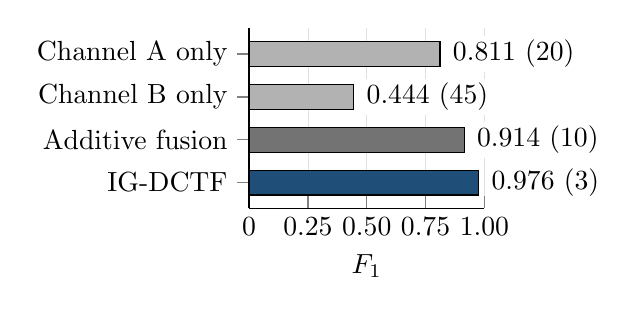
\begin{tikzpicture}
\begin{axis}[
    width=130pt, height=110pt,
    xbar, bar width=9pt,
    xmin=0, xmax=1.0, ymin=-0.6, ymax=3.6,
    xtick={0,0.25,0.5,0.75,1.0},
    xticklabels={0,0.25,0.50,0.75,1.00},
    xlabel={$F_1$},
    ytick={0,1,2,3},
    yticklabels={Channel A only,Channel B only,Additive fusion,IG-DCTF},
    y dir=reverse,
    axis x line*=bottom, axis y line*=left,   % no right/top frame: it ran through the value labels
    xmajorgrids, grid style={black!12,line width=0.3pt},
    axis line style={line width=0.5pt}, tick style={line width=0.5pt},
    clip=false,
]
  % bar shift=0pt keeps every single-bar plot centred on its own y position
  \addplot[xbar,bar shift=0pt,fill=black!30,draw=black,line width=0.4pt] coordinates {(0.8113,0)};
  \addplot[xbar,bar shift=0pt,fill=black!30,draw=black,line width=0.4pt] coordinates {(0.4444,1)};
  \addplot[xbar,bar shift=0pt,fill=black!55,draw=black,line width=0.4pt] coordinates {(0.9138,2)};
  \addplot[xbar,bar shift=0pt,fill=acc,     draw=black,line width=0.4pt] coordinates {(0.9756,3)};

  % value and miss-count annotations to the right of each bar
  \node[anchor=west,inner sep=1.5pt,fill=white,xshift=3pt] at (axis cs:0.8113,0) {0.811 (20)};
  \node[anchor=west,inner sep=1.5pt,fill=white,xshift=3pt] at (axis cs:0.4444,1) {0.444 (45)};
  \node[anchor=west,inner sep=1.5pt,fill=white,xshift=3pt] at (axis cs:0.9138,2) {0.914 (10)};
  \node[anchor=west,inner sep=1.5pt,fill=white,xshift=3pt] at (axis cs:0.9756,3) {0.976 (3)};
\end{axis}
\end{tikzpicture}
}}

\clearpage
{\noindent\textbf{fig10\_decision\_map.tex}\hfill\textit{one column (3.5 in)}\par\medskip
{
\footnotesize
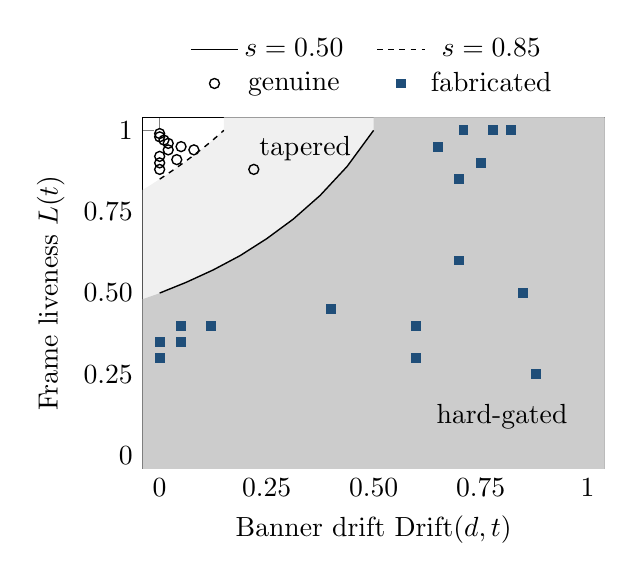
\begin{tikzpicture}
\begin{axis}[
    width=212pt, height=172pt,
    xmin=-0.04, xmax=1.04, ymin=-0.04, ymax=1.04,
    xtick={0,0.25,0.5,0.75,1}, xticklabels={0,0.25,0.50,0.75,1},
    ytick={0,0.25,0.5,0.75,1}, yticklabels={0,0.25,0.50,0.75,1},
    xlabel={Banner drift $\mathrm{Drift}(d,t)$},
    ylabel={Frame liveness $L(t)$},
    axis line style={line width=0.5pt}, tick style={line width=0.5pt},
    legend style={at={(0.5,1.03)},anchor=south,legend columns=2,draw=none,
                  /tikz/every even column/.append style={column sep=10pt}},
    clip=true,
]
  % tapered region: s < 0.85
  \addplot[fill=black!6,draw=none,forget plot] coordinates {
    (-0.040,-0.040) (1.040,-0.040) (1.040,1.040) (0.150,1.040) (0.150,1.000) (0.136,0.984) (0.123,0.969)
    (0.109,0.954) (0.096,0.940) (0.082,0.926) (0.069,0.913) (0.055,0.899) (0.041,0.887) (0.028,0.874)
    (0.014,0.862) (0.001,0.851) (-0.013,0.839) (-0.026,0.828) (-0.040,0.817)} -- cycle;
  % hard-gated region: s < 0.50
  \addplot[fill=black!20,draw=none,forget plot] coordinates {
    (-0.040,-0.040) (1.040,-0.040) (1.040,1.040) (0.500,1.040) (0.500,1.000) (0.461,0.928) (0.423,0.866)
    (0.384,0.812) (0.346,0.764) (0.307,0.722) (0.269,0.684) (0.230,0.649) (0.191,0.618) (0.153,0.590)
    (0.114,0.565) (0.076,0.541) (0.037,0.519) (-0.001,0.499) (-0.040,0.481)} -- cycle;

  % iso-curves (named in the legend instead of labelled in the plot)
  \addplot[black,line width=0.5pt] coordinates {
    (0.000,0.500) (0.062,0.533) (0.125,0.571) (0.188,0.615) (0.250,0.667) (0.312,0.727)
    (0.375,0.800) (0.438,0.889) (0.500,1.000)};
  \addplot[black,line width=0.5pt,dash pattern=on 2pt off 2pt] coordinates {
    (0.000,0.850) (0.025,0.872) (0.050,0.895) (0.075,0.919) (0.100,0.944) (0.125,0.971) (0.150,1.000)};

  % genuine scenarios
  \addplot[only marks,mark=o,mark size=1.8pt,line width=0.5pt,mark options={fill=white,draw=black}] coordinates {
    (0.00,0.98) (0.05,0.95) (0.00,0.92) (0.02,0.96) (0.00,0.90) (0.04,0.91)
    (0.01,0.97) (0.00,0.88) (0.00,0.99) (0.02,0.94) (0.08,0.94) (0.22,0.88)};
  % fabricated scenarios
  \addplot[only marks,mark=square*,mark size=1.6pt,mark options={fill=acc,draw=acc}] coordinates {
    (0.75,0.90) (0.65,0.95) (0.00,0.35) (0.05,0.40) (0.70,0.85) (0.40,0.45) (0.60,0.40) (0.85,0.50)
    (0.00,0.30) (0.60,0.30) (0.82,1.00) (0.78,1.00) (0.71,1.00) (0.00,0.30) (0.05,0.35) (0.12,0.40)
    (0.88,0.25) (0.70,0.60)};
  \legend{$s=0.50$, $s=0.85$, genuine, fabricated}

  % region labels (white = nominal, light grey = tapered, dark grey = hard-gated)
  \node[anchor=center] at (axis cs:0.80,0.12) {hard-gated};
  \node[anchor=center] at (axis cs:0.34,0.945) {tapered};
\end{axis}
\end{tikzpicture}
}}

\end{document}
